\chapter{ML-based FF for Alanine dipeptide in implicit solvent}

\section{Introduction: what we will do in this tutorial}
\begin{itemize}
\item Construct the system.
\item Perform biased molecular dynamics simulations using a classical force field ([ff14SBonlysc]) based potential to obtain samples. The bias is provided by [metadynamics], which is an adaptive potential of mean force technique.
\item Compute energy and atomic forces of collected configurations using a more expensive semiempirical potential ([PM6]).
\item Fit (learn) the PM6 potential energy surface by Gaussian process regression (GPR) and neural network (NN).
\item Perform molecular dynamics simulations on the ML-based potential energy surface.
\item Compute the free energy surface.
\end{itemize}





\paragraph{Before starting: create a conda virtual environment}
Make new virtual environment is a good habit to avoid messing up with packages. 
The best option is to use \texttt{conda}. This is heavier than the standard Python venv,
but is recommended because it provides more isolation. First, download Miniconda. Then navigate to the desired folder and run:

\begin{verbatim}
conda create -n ml_forcefields -c conda-forge python=3.11 
    ambertools ipykernel
\end{verbatim}
This creates a new virtual environemnt called \texttt{ml\_forcefields} and installs python,
ambertools and ipykernel within it. Now you need to enter it:
\begin{verbatim}
conda activate ml_forcefields
\end{verbatim}
and install all the packages you need within it (e.g. pip, torch etc). In order to use
the the virtual environment interpreter with VSCode, you need to register
the kernel:
\begin{verbatim}
 python -m ipykernel install --user --name ml_forcefields --display-name
     "Python (ml_forcefields)"
\end{verbatim}
Then you open VSCode and change your kernel to that. If you want to exit the virtual environment,
simply type \texttt{conda deactivate}.


\paragraph{Implicit solvent simulations:} A simulation in implicit solvent is a molecular dynamics (MD) approach where the solvent (usually water) is not represented by individual molecules, but instead treated as a continuous medium.
Instead of simulating thousands of explicit water molecules, the solvent’s effect is modeled mathematically—mainly through dielectric screening (reducing electrostatic interactions)
and effective solvation energies (penalizing or favoring exposure to solvent). Advantages are that these simulations
are much faster and therefore are useful for sampling large conformational changes. However, they dont allow for a detailed representation
of the solvent's structure (e.g. hydrogen bonds, water networks) and are less accurate for fine-grained interactions. 

\paragraph{The alanine dipeptide}
Alanine dipeptide (often \(N\)-acetyl-L-alanyl-methylamide) is a small molecule consisting of a central alanine residue capped by acetyl and methylamino groups.
Is the go-to toy example for studying conformational space kinetics  because it captures the essentials of peptide conformational behavior while staying extremely simple.
It is almost entirely described by just two dihedral angles, which makes it ideal for visualizing free energy landscapes (Ramachandran plots).
Also it exhibits a few clear conformations (e.g. $\alpha$ basins, $\beta$ basins), separated by barriers. This makes it perfect for studying
transition kinetics and testing enhanced sampling methods.
\begin{figure}[H]
    \centering
    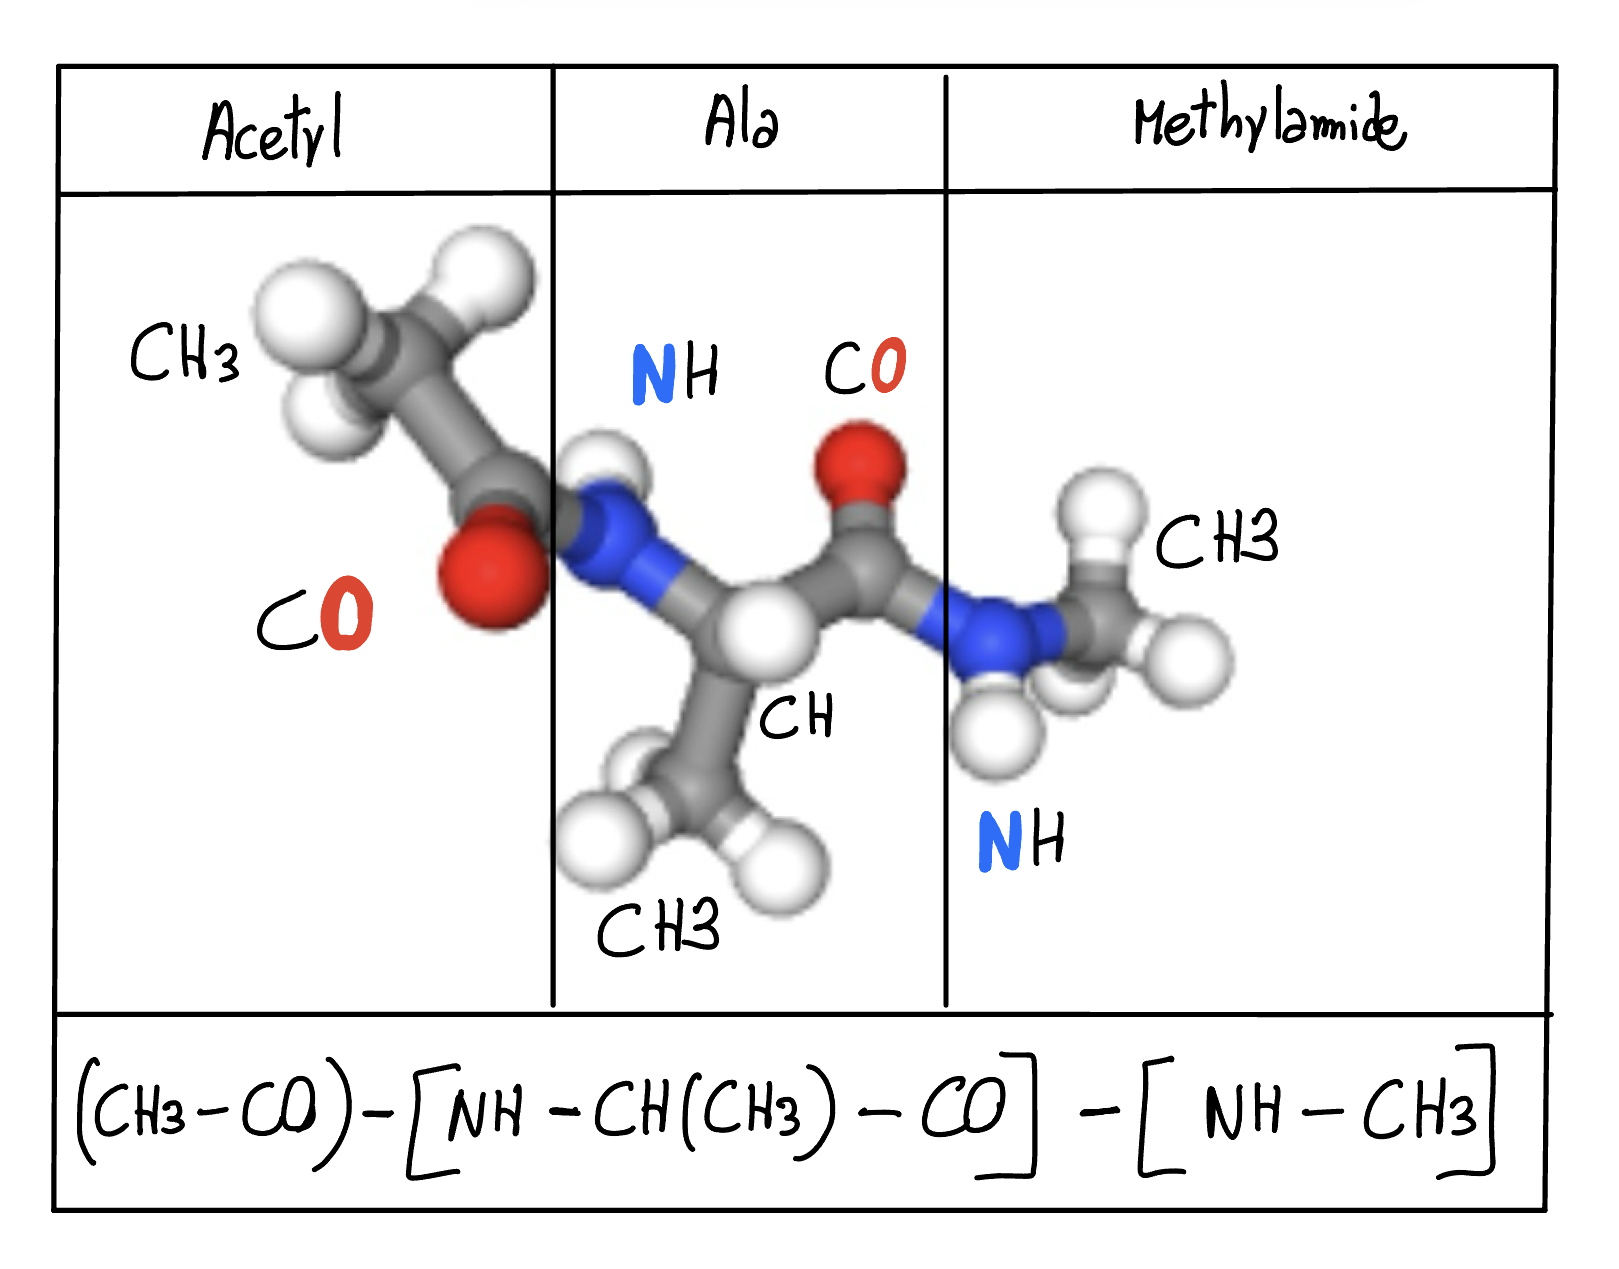
\includegraphics[width = 0.48\textwidth]{img_alanine/alanine_formula.png}
    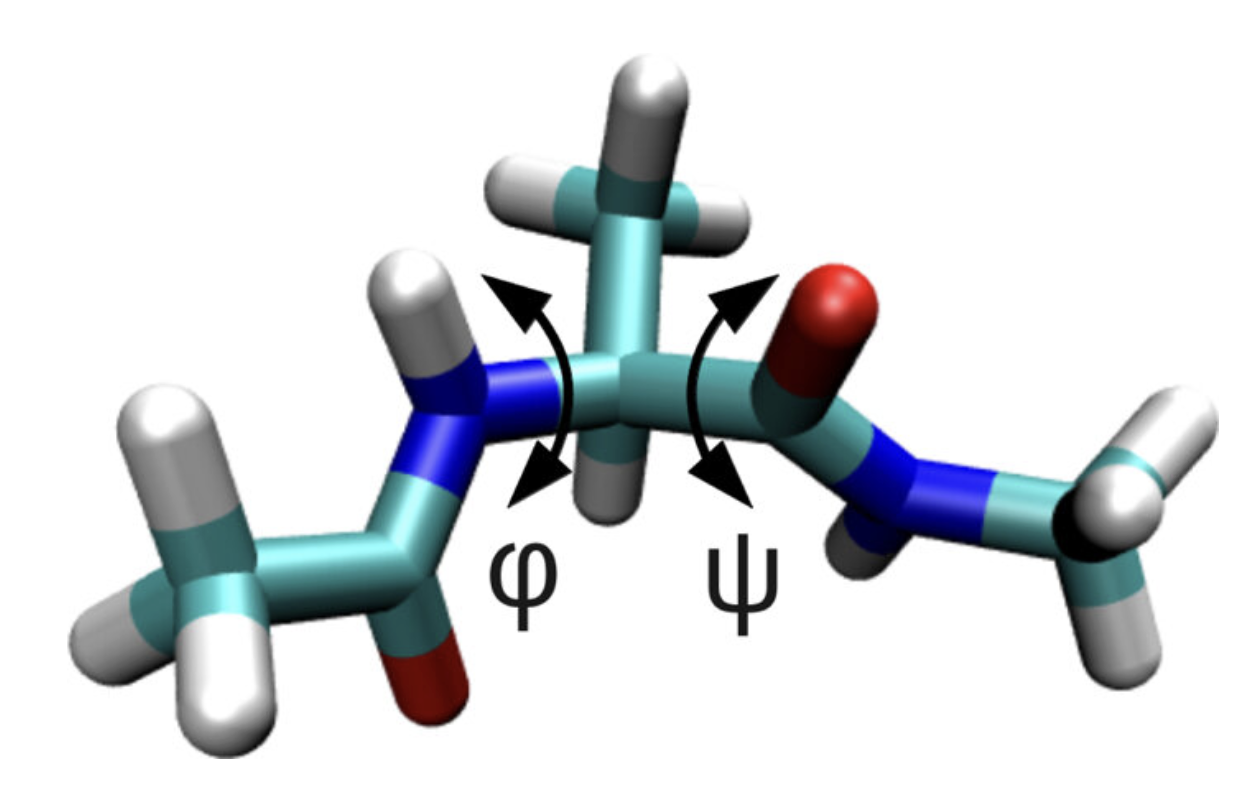
\includegraphics[width = 0.48\textwidth]{img_alanine/alanine_angles.png}
    \caption{The two dihedrals $\phi$ and $psi$ are the collective variables (CVs) of the alanine dipeptide.}
\end{figure}

\newpage

\section{Glossary of essential notions}
\paragraph{Basic notations:}

\begin{itemize}
    \item $\mathbf{x}, \, \mathbf{p}$: cartesian coordinates and momenta.
    \item \textbf{Configuration or microstate:} a single spatial arrangement of particles, represented by coordinates $\mathbf{x}$.
    \item \textbf{Configuration space, $\Gamma$:} The set of possible configurations.
    \item \textbf{Phase space:} the configuration space augmented with the momenta variables.
    \item \textbf{Hamiltonian:} $H(x,p) = U(x) + K(p)$ is a sum of the potential energy function denoted by $U(x)$, defined by a classical molecular mechanics force field, and the kinetic energy $K(p)$.
    \item \textbf{Hamiltonian dynamics:} 
    $$
    \begin{cases}
    d\mathbf{x} &= M^{-1}\,\mathbf{p}\,dt \\
    d\mathbf{p} &= -\nabla_x \,U(\mathbf{x})\,dt
    \end{cases}
    $$
\end{itemize}

\noindent Hamiltonian dynamics conserves mechanical energy, and can be used to sample from the microcanonical (constant number of particles N, constant volume V and constant energy E, NVE) ensemble under an ergodicity assumption.
Isothermal dynamics includes modifications that function as a thermostat, simulating the equilibrium with an external temperature bath at a target temperature T. 
As a result, as long as the simulation is at or near equilibrium, its temperature fluctuates around T, and it samples the canonical ensemble (NVT).

\paragraph{Canonical ensemble probability density of \textit{microstates}}
The phase space probability density is given by:

$$
\mu(\mathbf{x}, \mathbf{p}) = \frac{1}{Q} e^{-\beta U(\mathbf{x}) + K(\mathbf{p})},
$$

where

$$
Q = \int e^{-\beta (U(\mathbf{x}) + K(\mathbf{p}))} \, d\mathbf{x} \, d\mathbf{p}
$$

is the normalization factor, known as the partition function. In most cases, the energy is a sum of a potential term that depends only on positions and a kinetic term that depends only on momenta. The momenta are statistically independent from the system configuration, hence their distribution is that of the ideal gas and does not bear significant information on any specific system. This leads to a simple expression for the configurational distribution, where the momenta and kinetic energy do not appear:

$$
\rho(\mathbf{x}) = \int \mu(\mathbf{x}, \mathbf{p}) \, d\mathbf{p} = \frac{1}{Z} e^{-\beta U(\mathbf{x})},
$$

where $Z$ is the \textbf{configurational} partition function:

$$
Z = \int e^{-\beta U(\mathbf{x})} \, d\mathbf{x}.
$$


\paragraph{Macrostates}

Macrostates are experimentally distinguishable or measurable states of a system. They can be described formally either in terms of thermodynamic state variables $(E, T, P, V)$, or parameters of the Hamiltonian, or by specifying regions of configuration space $\Sigma$ (that is, disjoint sets of microstates).
The probability of a region of phase space $\Sigma$ is:

$$
P(\Sigma) = \int_{\Sigma} \mu(\mathbf{x}, \mathbf{p}) \, d\mathbf{x} \, d\mathbf{p} = \frac{Z(\Sigma)}{Z}
$$

\paragraph{Free energy, F}
A single scalar number associated with the canonical ensemble:

$$
F(T, V, N) = - k_B\,T \ln{Z}*
$$
(* or should it be $\ln{Q}$, to include also the velocities ?.)


\paragraph{Free energy \textit{of a macrostate}} similarly, defined as

$$
F(\Sigma) = - k_B\,T \ln{Z(\Sigma)}
$$
hence, the probability ratio of two macrostates $\Sigma_A, \Sigma_B$ is linked to their free energy difference:

$$
\Delta F = - k_B T \ln{\frac{P_A}{P_B}}.
$$

\paragraph{Collective Variable (CV)}

A collective variable is a function $\xi$ mapping the full $n$-dimensional configuration $\mathbf{x}$ to a lower-dimensional representation $\mathbf{z}$ (sometimes denoted as $\mathbf{s}$ in the literature):
$$
\mathbf{z} = \xi(\mathbf{x}).
$$
\paragraph{Dimensionality Reduction}

Dimensionality reduction is the process of finding functions $\xi$ that map high-dimensional configurations $\mathbf{x}$ to low-dimensional representations $\mathbf{z}$.

\paragraph{Free Energy Surface (FES)}

While free energy can be expressed as the logarithm of a partition function, a free energy surface (FES) is the logarithm of a partially integrated partition function.

Given a chosen set of collective variables $\mathbf{z} = \xi(\mathbf{x})$, this partially integrated partition function corresponds, up to a normalization factor, to the marginal probability density $\rho(\mathbf{z})$. It is obtained by integrating the Boltzmann density over all variables except $\mathbf{z}$ (at fixed $\mathbf{z}$):
$$
A(\mathbf{z}) = -\beta^{-1} \ln \int \delta(\mathbf{z} - \xi(\mathbf{x})) \, \mu(\mathbf{x}) \, d\mathbf{x}
= -\beta^{-1} \ln \rho(\mathbf{z}).
$$



\begin{figure}[H]
    \hrule
    \centering
    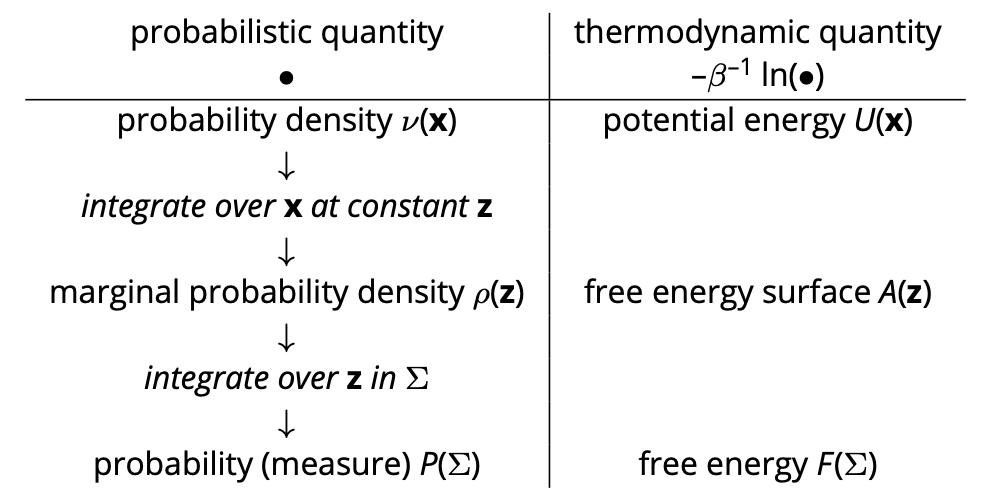
\includegraphics[width = \textwidth]{img_alanine/delemotte.png}
    \hrule
    \vspace*{20pt}
    \caption{Relations between key statistical and thermodynamics quantities. The right column is $\beta^{-1}$  times the logarithm of the left colunm.Probabilistic quantities are related by successive integration over larger slices of configuration space. Taken from: Henin, J., Lelievre, T., Delemotte, L., "Enhanced sampling methods for molecular dynamics simulations".  }
\end{figure}




\paragraph{Important remark: FES maxima are NOT necessarily kinetic barriers}
The free energy surface can be interpreted as an effective potential energy surface defined on collective variables.
But, importantly, free energy surfaces do not generally have a simple interpretation in terms of dynamics.
For example, free energy maxima are not necessarily kinetic barriers, due to distortions arising from the nonlinear geometry of the chosen collective variables.




\paragraph{The link between CV-based ehnanced sampling methods and dimensionality reduction}











\newpage
\section{Notebook walk-through (the physics side)}
Let's first discard the ML layer and focus on the key physical concepts underlying the proposed workflow. This
notebook basically demostrates a standard workflow behind modern MD simulations. The goal is \textbf{exploration of the conformational ensemble} of
the system (here, alanine dipeptide). Consider that we are in the NVT ensemble.


\paragraph{First step: unbiased simulation}
An unbiased simulation is just standard molecular dynamics evolving under the physical Hamiltonian:

$$
m_i \ddot{\mathbf{R}}_i = - \nabla_i V(\mathbf{R})
$$

where $ V(\mathbf{R})$ is the potential energy surface (PES). Ideally, if run long enough (and assuming ergodicity),
this simulation samples the Boltzmann distribution:

$$
P(\mathbf{R}) \propto e^{-\beta V(\mathbf{R})}
\quad \text{with} \quad \beta = \frac{1}{k_B T}
$$

Lower the energy of a state, higher is the probability of visiting it. Also we need to consider energy barriers separating states.

In practice, however, we can never run a simulation long enough to explore the whole conformational space. 

(Why would we want to explore the conformational space?
Because there are conformational states of the biomolecule that we may desire to exploit for drug design, e.g. modulate the biomolecule
so that those states- which are very rare and unstable in the wild type - become more stable. ) Often, it will get trapped in one basin (one metastable configuration) and never get out of that. It will not sample rare transitions.

\begin{figure}[H]
    \centering
    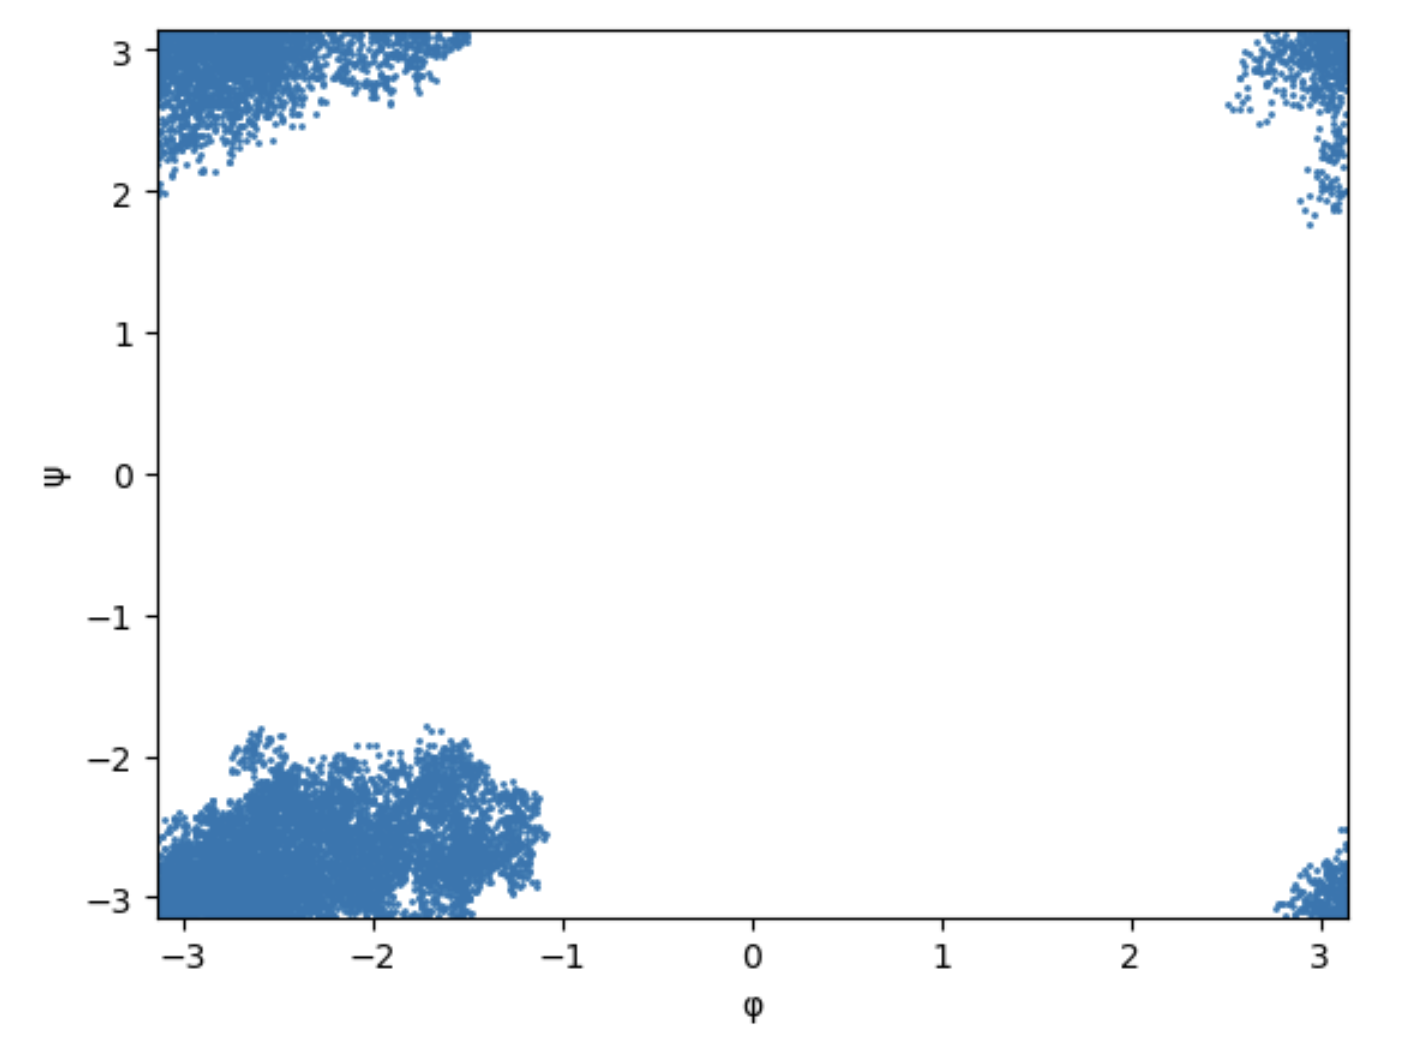
\includegraphics[width = 0.8\textwidth]{img_alanine/unbiased_sim.png}
    \caption{Scatterplot of the states visited in the unbiased simulation. Just one metastable state is visited.}
\end{figure}

\paragraph{Second step: simulation with enhanced sampling (metadynamics)}


So we want to \textbf{bias} the simulation to \textbf{force exploration} of the phase space. There are a lot of different techniques for that,
which broadly are referred to as \textbf{enhanced sampling techniques}. In this tutorial, we use \textbf{metadynamics}. 

The core idea of metadynamics is to add a history-dependent bias to force exploration of phase space. Instead of evolving with $V(\mathbf{R})$, you evolve with:

$$
V_{\text{total}}(\mathbf{R}, t) = V(\mathbf{R}) + V_{\text{bias}}(s(\mathbf{R}), t)
$$

where $s(\mathbf{R})$ are the collective variables. The bias term $V_{bias}$ is constructed as a sum of Gaussians is deposited along the trajectory:

$$
V_{\text{bias}}(s,t) = \sum_{t' < t} w \exp\left( -\frac{(s - s(t'))^2}{2\sigma^2} \right)
$$

Interpretation: each time the system visits a region, you discourage revisiting it (you "fill" the energy wells). The barriers
are progressively flattened and the system is pushed to explore new states.

\begin{figure}[H]
    \centering
    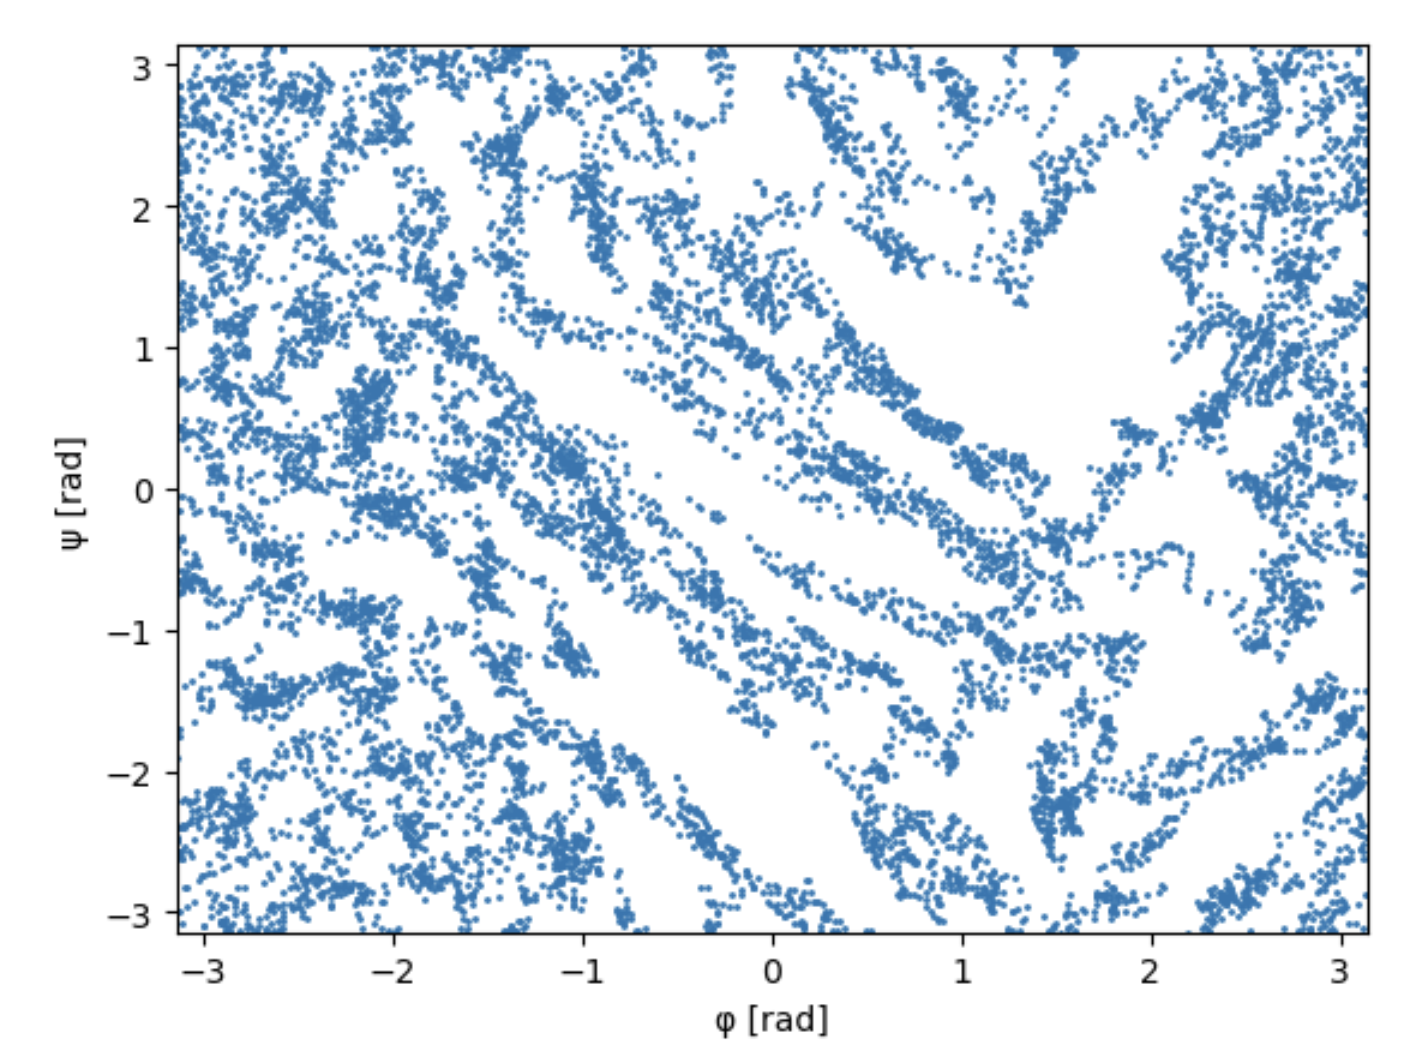
\includegraphics[width = 0.8\textwidth]{img_alanine/metadyn_sim.png}
    \caption{Scatterplot of the states visited in the metadynamics simulation. A pletora of states appear.}
\end{figure}




\paragraph{Third step: reconstruction of the Free Energy Surface}

The free energy as a function of CVs is:

$$
F(s) = -k_B T \ln P(s)
$$


\begin{figure}[H]
    \centering
    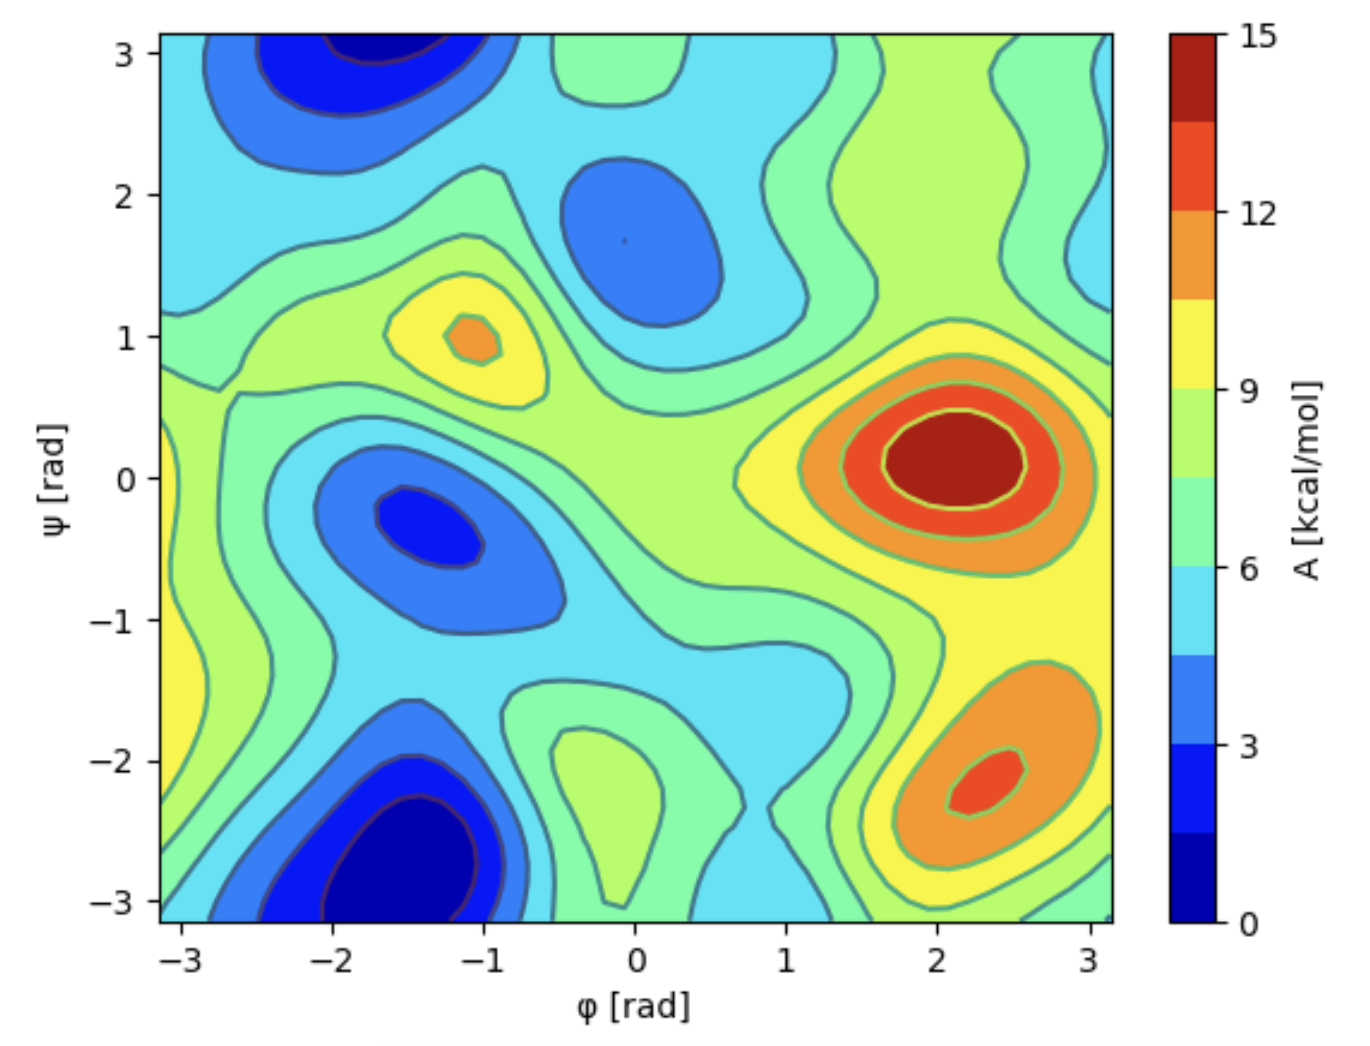
\includegraphics[width = 0.8\textwidth]{img_alanine/free_surface.png}    
    \caption{Reconstructed free energy surface.}
\end{figure}


\section{Notebook walk-through: (the ML side)}